\documentclass[a4paper,10pt]{article}
\usepackage[utf8]{inputenc}
\usepackage{datetime}
\usepackage{listings}
\usepackage{graphicx}
\newdate{date}{24}{03}{2017}
\date{\displaydate{date}}

\title{Homework 2\\Marlen Akimaliev\\BIL622-Numerical Analysis II}
%\author{Share\LaTeX}

\begin{document}

\maketitle

\section{Problem}
Given the differential equation $y'=(y+x)^2$ with initial condition $y(0)=0$ at the interval $[0, 0.5]$, find the solution using Euler method with $h=0.1$. Compare results with the solution of the equation given by $y = tan(x)-x$.
\section{Solution}
Solution for 6 points as a table in the interval $[0, 0.5]$ is as follows:
\begin{center}
\begin{tabular}{ |c|c| } 
 \hline
 $x$ & $y$\\
\hline
 $0.0$ & $0.0000000000000000$\\
 $0.1$ & $0.0000000000000000$\\
 $0.2$ & $0.0010000000000000$\\
 $0.3$ & $0.0050401000000000$\\
 $0.4$ & $0.0143450462608010$\\
 $0.5$ & $0.0315132279968875$\\
 \hline
\end{tabular}
\end{center}
We can use the following expression to evaluate the absolute error, which is the sum of the absolute values of the residuals:\\
$$\varepsilon_{abs} = \sum_{i=1}^{N} |y(x_i)-w_i|$$\\
I have used the following Python code \cite{connor} to evaluate values and plot the graph.
\begin{lstlisting}[language=Python]
import numpy as np
from matplotlib import pyplot as plt
def euler( f, x0, y0, x1, n):
	# determine step-size
	h = (x1-x0)/float(n)             
	t = np.arange(x0, x1+h, h )         
	w = np.zeros((n+1,))                     
	t[0] = x0
	w[0] = y0   
	for i in range(1,n+1):                       
		w[i] = w[i-1] + h * f(t[i-1], w[i-1])
		t[i] = x0 + i * h
	return t,w
def f(x,y): return (y+x)**2
def y(x): return np.tan(x)-x
vx,vy = euler(f, 0, 0, 0.5, 5)
yx = []
for v in vx:
	yx.append(y(v))
dummy, w = euler(f, 0, 0, 0.5, 5)
error_abs = lambda y, w: np.sum(np.abs(y - w))
err = error_abs(yx, w)
print err
for x, y in list(zip(vx, vy))[::1]:
    print("%4.1f %10.16f" % (x, y))
plt.plot(vx, vy, label='approximation')
plt.plot( vx, yx, label='exact' )
plt.title( "Euler's Method Example")
plt.xlabel('Value of x') 
plt.ylabel('Value of y')
\end{lstlisting}
Error value equals to $0.029578291528$.\\
If we try to plot these values and the exact function as a graph result is as follows:
\begin{figure}[ht]
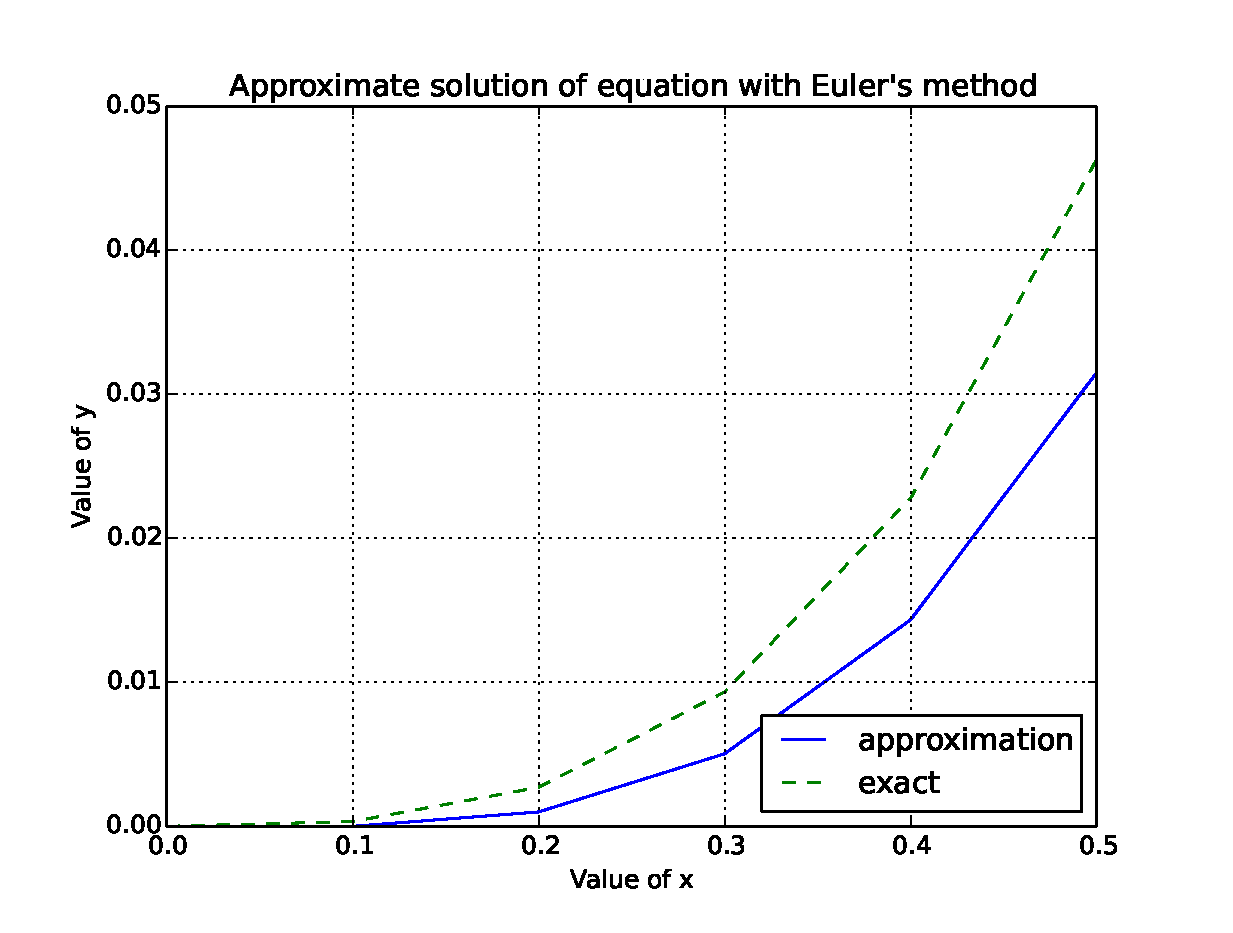
\includegraphics[width=8cm]{1_1.eps}
\end{figure}

\medskip

\begin{thebibliography}{9}
\bibitem{connor} Numerical Solutions to ODEs, \\\texttt{http://connor-johnson.com/2014/02/21/numerical-solutions-to-odes/}
\end{thebibliography}

\end{document}
